\documentclass[11pt,a4paper]{article}

\usepackage[a4paper,margin=0.85in]{geometry}
\usepackage{booktabs}
\usepackage{array}
\usepackage{longtable}
\usepackage{multirow}
\usepackage{graphicx}
\usepackage{xcolor}
\usepackage{hyperref}
\usepackage{tikz}
\usepackage{pgfplots}
\usepackage{pgfplotstable}
\usepackage{caption}
\usepackage{subcaption}
\usepackage{float}
\usepackage{enumitem}
\usepackage{fancyhdr}
\usepackage{listings}
\usepackage{mdframed}
\usepackage{microtype}
\usepackage{parskip}

\usetikzlibrary{arrows.meta,positioning,fit,shapes.geometric,shapes.misc,calc,backgrounds}
\pgfplotsset{compat=1.18}

%% ── Colour palette ──────────────────────────────────────────────────────────
\definecolor{vsblue}{RGB}{34,83,140}
\definecolor{vsgreen}{RGB}{40,135,92}
\definecolor{vsorange}{RGB}{209,110,35}
\definecolor{vsred}{RGB}{180,55,55}
\definecolor{vslight}{RGB}{241,245,249}
\definecolor{vsgray}{RGB}{80,88,100}
\definecolor{vsdark}{RGB}{20,40,70}
\definecolor{vspurple}{RGB}{120,60,160}

\hypersetup{
  colorlinks=true,
  linkcolor=vsblue,
  urlcolor=vsblue,
  citecolor=vsblue
}

%% ── Header / footer ─────────────────────────────────────────────────────────
\pagestyle{fancy}
\setlength{\headheight}{14pt}
\fancyhf{}
\lhead{\textcolor{vsblue}{\textbf{VecScaleDB}}}
\rhead{\textcolor{vsgray}{Distributed Vector Database Report}}
\cfoot{\thepage}

%% ── Code listings ───────────────────────────────────────────────────────────
\lstset{
  basicstyle=\ttfamily\scriptsize,
  breaklines=true,
  breakatwhitespace=false,
  postbreak=\mbox{\textcolor{vsblue}{$\hookrightarrow$}\space},
  frame=single,
  rulecolor=\color{vsblue!40},
  backgroundcolor=\color{vslight},
  columns=fullflexible,
  keepspaces=true,
  showstringspaces=false,
  xleftmargin=4pt,
  xrightmargin=4pt
}

%% ── Box style for highlights ────────────────────────────────────────────────
\newmdenv[
  linecolor=vsblue,
  linewidth=1.2pt,
  backgroundcolor=vslight,
  innerleftmargin=10pt,
  innerrightmargin=10pt,
  innertopmargin=6pt,
  innerbottommargin=6pt
]{infobox}

%% ── Shared TikZ styles ──────────────────────────────────────────────────────
\tikzset{
  vsbox/.style={draw=vsblue!70, rounded corners=4pt, fill=vslight,
                align=center, text=vsdark, font=\small,
                minimum width=2.4cm, minimum height=0.8cm, thick},
  vscoord/.style={draw=vsblue, rounded corners=4pt, fill=vsblue!15,
                  align=center, text=vsdark, font=\small\bfseries,
                  minimum width=2.5cm, minimum height=0.85cm, thick},
  vswriter/.style={draw=vsgreen, rounded corners=4pt, fill=vsgreen!10,
                   align=center, text=vsdark, font=\small\bfseries,
                   minimum width=2.4cm, minimum height=0.85cm, thick},
  vsreader/.style={draw=vsorange, rounded corners=4pt, fill=vsorange!10,
                   align=center, text=vsdark, font=\small\bfseries,
                   minimum width=2.2cm, minimum height=0.8cm, thick},
  vsstorage/.style={draw=vspurple!70, cylinder, shape border rotate=90,
                    aspect=0.22, fill=vspurple!10, align=center,
                    text=vsdark, font=\small,
                    minimum height=1.1cm, minimum width=1.6cm, thick},
  arrow/.style={-{Latex[length=2.5mm,width=1.6mm]}, thick, color=vsblue},
  arrowg/.style={-{Latex[length=2.5mm,width=1.6mm]}, thick, color=vsgreen},
  arrowmeta/.style={-{Latex[length=2.5mm,width=1.6mm]}, thick, dashed, color=vsorange},
  flowstep/.style={draw=vsblue!60, rounded corners=4pt, fill=vslight,
                   align=center, text=vsdark, font=\small,
                   minimum width=2.8cm, minimum height=0.9cm, thick},
  decision/.style={draw=vsorange, diamond, fill=vsorange!10,
                   align=center, text=vsdark, font=\footnotesize,
                   minimum width=1.8cm, minimum height=0.8cm, thick},
}

%% ── Title ───────────────────────────────────────────────────────────────────
\title{%
  \vspace{-1em}%
  {\color{vsblue}\rule{\linewidth}{2pt}}\\[6pt]
  \textbf{\Large VecScaleDB: Distributed Vector Database}\\[4pt]
  \large Architecture, Feature Validation, Dataset Evaluation,\\
  and Benchmark Report\\[4pt]
  \normalsize Repository: \href{https://github.com/sanchit-22/Distributed-Vector-DB}{github.com/sanchit-22/Distributed-Vector-DB}\\[6pt]
  {\color{vsblue}\rule{\linewidth}{0.8pt}}
}
\author{%
  \textbf{Team Deadlock and Chill}\\[4pt]
  Sanchit Kumar -- 2024201042\\
  Priyanshu Jha -- 2024201062\\
  Rohini Mandlekar -- 2025901004
}
\date{4th May 2026}

%%%%%%%%%%%%%%%%%%%%%%%%%%%%%%%%%%%%%%%%%%%%%%%%%%%%%%%%%%%%%%%%%%%%%%%%%%%%
\begin{document}
\maketitle
\thispagestyle{fancy}

\begin{abstract}
VecScaleDB is a distributed vector database engineered from scratch for a
distributed-systems course project. It separates the concerns of metadata
coordination, write ingestion, immutable segment storage, and stateless reader
execution. The system uses a WAL-backed LSM-style storage engine, FAISS
IVF\_FLAT segment indexes, shared-storage segment files, and coordinator-driven
routing with scatter-gather and replicated search modes. This report documents
the system architecture, all request flows, dataset configuration, benchmark
methodology, measured results, and the test strategy used to validate the
features promised in the project proposal.
\end{abstract}

\tableofcontents
\newpage

%%%%%%%%%%%%%%%%%%%%%%%%%%%%%%%%%%%%%%%%%%%%%%%%%%%%%%%%%%%%%%%%%%%%%%%%%%%%
\section{Executive Summary}

VecScaleDB implements a WAL-backed LSM-style vector storage engine, FAISS
IVF\_FLAT segment indexes, shared-storage segment files, coordinator metadata
routing, writer ingestion, reader-side segment caching, scatter-gather search,
and replicated reader benchmark mode. A fresh proposal-level feature test suite
plus a comprehensive unit and integration suite validate all core mechanisms.

\begin{table}[H]
\centering
\caption{Implementation status against proposal features.}
\renewcommand{\arraystretch}{1.2}
\begin{tabular}{>{\bfseries}p{0.27\linewidth} p{0.13\linewidth} p{0.50\linewidth}}
\toprule
Feature & Status & Evidence \\
\midrule
Distributed and scalable architecture & \textcolor{vsgreen}{Done} &
  Coordinator ring, writer, readers, shared storage, etcd, sharding, and
  5-reader Docker topology. \\
Vector similarity search & \textcolor{vsgreen}{Done} &
  IVF\_FLAT segment indexes with external IDs, top-k search, and nprobe
  control. \\
Dynamic data management & \textcolor{vsgreen}{Done} &
  Insert, delete (tombstones), MemTable flush, immutable segments, and
  reinsert-as-update semantics. \\
Snapshot isolation & \textcolor{vsgreen}{Done} &
  Search visibility filtered by snapshot ID across MemTable and segments. \\
Fault tolerance & \textcolor{vsgreen}{Done} &
  WAL recovery, shared-storage reader reload, coordinator TTL election, and
  coordinator-client failover. \\
Distributed 5-node cluster & \textcolor{vsgreen}{Done} &
  Docker Compose: 3 coordinators, 1 writer, 5 readers, etcd. \\
\bottomrule
\end{tabular}
\end{table}

%%%%%%%%%%%%%%%%%%%%%%%%%%%%%%%%%%%%%%%%%%%%%%%%%%%%%%%%%%%%%%%%%%%%%%%%%%%%
\section{System Architecture}

\subsection{Component Overview}

The cluster follows a \emph{shared-storage} design. Compute nodes are
stateless or recoverable, while durability is provided by WAL files and
immutable segment files written to a host volume that all nodes can access.

\begin{table}[H]
\centering
\caption{Runtime roles and responsibilities.}
\renewcommand{\arraystretch}{1.2}
\begin{tabular}{p{0.16\linewidth} p{0.18\linewidth} p{0.56\linewidth}}
\toprule
\textbf{Role} & \textbf{Count} & \textbf{Responsibility} \\
\midrule
Coordinator & 3 replicas &
  Maintains node registrations, segment metadata, leader state, current
  snapshot metadata, routing, and search fanout policy. \\
Writer & 1 process &
  Accepts inserts/deletes, appends WAL records, updates the MemTable,
  flushes immutable segments, and registers segment metadata with the
  coordinator. \\
Reader & 1–5 processes &
  Refreshes segment metadata, loads assigned or replicated segments from
  shared storage, searches its local segment cache, and returns partial
  top-k results to the coordinator. \\
Shared storage & Host volume &
  Stores \texttt{index.faiss}, \texttt{ids.npy}, \texttt{vectors.npy},
  \texttt{meta.json}, \texttt{tombstones.json}, and WAL files. \\
etcd & 1 service &
  Provides a metadata store and coordinator leader election via TTL
  campaigns. \\
\bottomrule
\end{tabular}
\end{table}

\subsection{Port Map}

\begin{table}[H]
\centering
\caption{Default port assignments in distributed Docker mode.}
\renewcommand{\arraystretch}{1.15}
\begin{tabular}{lll}
\toprule
\textbf{Service} & \textbf{Port} & \textbf{Key endpoints} \\
\midrule
Coordinator 0 & 8000 & \texttt{/search}, \texttt{/segments}, \texttt{/health}, \texttt{/metrics} \\
Coordinator 1 & 8001 & Same as coordinator 0 (replica) \\
Coordinator 2 & 8002 & Same as coordinator 0 (replica) \\
Writer 0       & 8100 & \texttt{/insert}, \texttt{/delete}, \texttt{/health}, \texttt{/metrics} \\
Reader 0       & 8200 & \texttt{/ready}, \texttt{/metrics} \\
Reader 1       & 8201 & \texttt{/ready}, \texttt{/metrics} \\
Reader 2       & 8202 & \texttt{/ready}, \texttt{/metrics} \\
Reader 3       & 8203 & \texttt{/ready}, \texttt{/metrics} \\
Reader 4       & 8204 & \texttt{/ready}, \texttt{/metrics} \\
\bottomrule
\end{tabular}
\end{table}

\subsection{Architecture Diagram}

\begin{figure}[H]
\centering
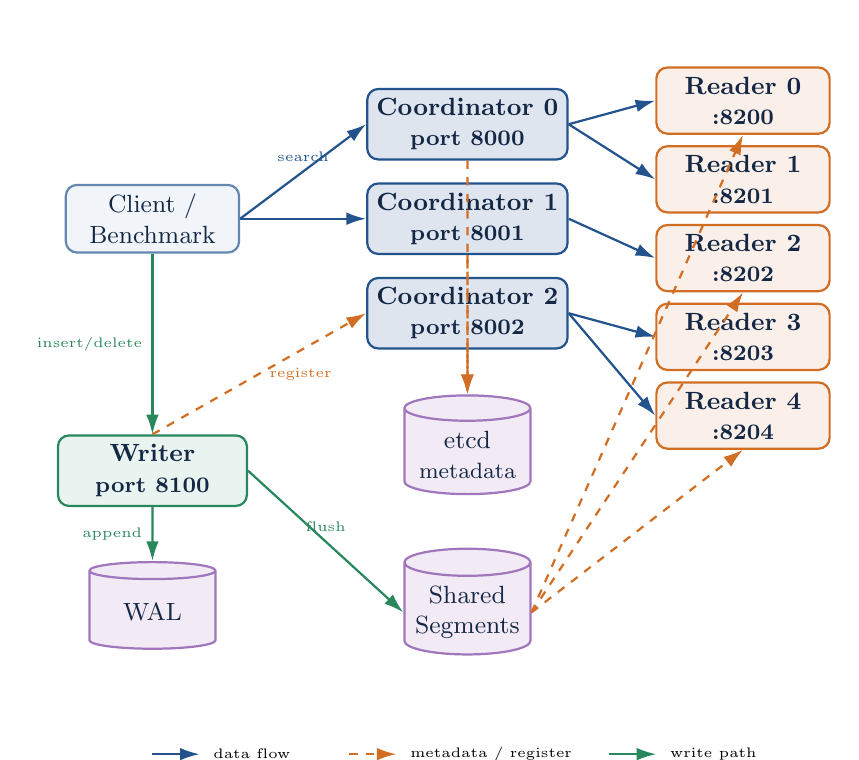
\begin{tikzpicture}[x=1cm, y=1cm]

  %% ── Client ──────────────────────────────────────────
  \node[vsbox, minimum width=2.2cm] (client) at (0, 0) {Client /\\Benchmark};

  %% ── Coordinators (stacked column) ───────────────────
  \node[vscoord] (c0) at (4, 1.2)  {Coordinator 0\\{\footnotesize port 8000}};
  \node[vscoord] (c1) at (4, 0)    {Coordinator 1\\{\footnotesize port 8001}};
  \node[vscoord] (c2) at (4,-1.2)  {Coordinator 2\\{\footnotesize port 8002}};

  %% ── etcd ────────────────────────────────────────────
  \node[vsstorage] (etcd) at (4, -3) {etcd\\{\footnotesize metadata}};

  %% ── Writer ──────────────────────────────────────────
  \node[vswriter] (writer) at (0,-3.2) {Writer\\{\footnotesize port 8100}};

  %% ── Storage ─────────────────────────────────────────
  \node[vsstorage] (wal)      at (0,-5.0) {WAL};
  \node[vsstorage] (segments) at (4,-5.0) {Shared\\Segments};

  %% ── Readers (spread horizontally) ───────────────────
  \node[vsreader] (r0) at (7.5, 1.5)  {Reader 0\\{\footnotesize :8200}};
  \node[vsreader] (r1) at (7.5, 0.5)  {Reader 1\\{\footnotesize :8201}};
  \node[vsreader] (r2) at (7.5,-0.5)  {Reader 2\\{\footnotesize :8202}};
  \node[vsreader] (r3) at (7.5,-1.5)  {Reader 3\\{\footnotesize :8203}};
  \node[vsreader] (r4) at (7.5,-2.5)  {Reader 4\\{\footnotesize :8204}};

  %% ── Edges ───────────────────────────────────────────
  %% client → coordinators
  \draw[arrow] (client.east) -- node[above,font=\tiny]{search} (c0.west);
  \draw[arrow] (client.east) -- (c1.west);

  %% client → writer
  \draw[arrowg] (client.south) -- node[left,font=\tiny]{insert/delete} (writer.north);

  %% coordinators ↔ etcd
  \draw[arrowmeta] (c0.south) -- (etcd.north);
  \draw[arrowmeta] (c1.south) -- (etcd.north);
  \draw[arrowmeta] (c2.south) -- (etcd.north);

  %% writer → WAL
  \draw[arrowg] (writer.south) -- node[left,font=\tiny]{append} (wal.north);

  %% writer → segments (flush)
  \draw[arrowg] (writer.east) -- node[above,font=\tiny]{flush} (segments.west);

  %% writer → coordinator (register)
  \draw[arrowmeta] (writer.north) -- node[right,font=\tiny]{register} (c2.west);

  %% coordinators → readers (fanout)
  \draw[arrow] (c0.east) -- (r0.west);
  \draw[arrow] (c0.east) -- (r1.west);
  \draw[arrow] (c1.east) -- (r2.west);
  \draw[arrow] (c2.east) -- (r3.west);
  \draw[arrow] (c2.east) -- (r4.west);

  %% segments → readers (load/cache)
  \draw[arrowmeta] (segments.east) -- (r0.south);
  \draw[arrowmeta] (segments.east) -- (r2.south);
  \draw[arrowmeta] (segments.east) -- (r4.south);

  %% ── Legend ──────────────────────────────────────────
  \begin{scope}[shift={(0,-6.8)}]
    \draw[arrow]     (0,0) -- (0.6,0); \node[right,font=\tiny] at (0.65,0) {data flow};
    \draw[arrowmeta] (2.5,0) -- (3.1,0); \node[right,font=\tiny] at (3.15,0) {metadata / register};
    \draw[arrowg]    (5.8,0) -- (6.4,0); \node[right,font=\tiny] at (6.45,0) {write path};
  \end{scope}
\end{tikzpicture}
\caption{VecScaleDB shared-storage architecture. Coordinators maintain metadata
and fan out search queries. The writer persists mutations and creates immutable
segments. Readers load segments on demand for search execution.}
\end{figure}

\subsection{Storage Layout}

Each flushed segment is immutable and self-contained. The on-disk layout is:

\begin{itemize}[noitemsep,topsep=4pt]
  \item \texttt{index.faiss} — serialised FAISS IVF\_FLAT index (or
    \texttt{IndexFlatL2} for tiny segments).
  \item \texttt{ids.npy} — external vector IDs as a NumPy array.
  \item \texttt{vectors.npy} — raw float32 vectors used for merge/compaction.
  \item \texttt{meta.json} — segment ID, shard ID, vector count, snapshot ID,
    creation timestamp, and storage path.
\end{itemize}

Deletes are stored as WAL records with operation type \texttt{OP\_DE\-LETE} and
are persisted in \texttt{tomb\-stones.json}. Both single-node search and
distributed readers filter tombstoned IDs before physical merge.

%%%%%%%%%%%%%%%%%%%%%%%%%%%%%%%%%%%%%%%%%%%%%%%%%%%%%%%%%%%%%%%%%%%%%%%%%%%%
\section{Request Flows}

\subsection{Insert and Delete Flow}

\begin{figure}[H]
\centering
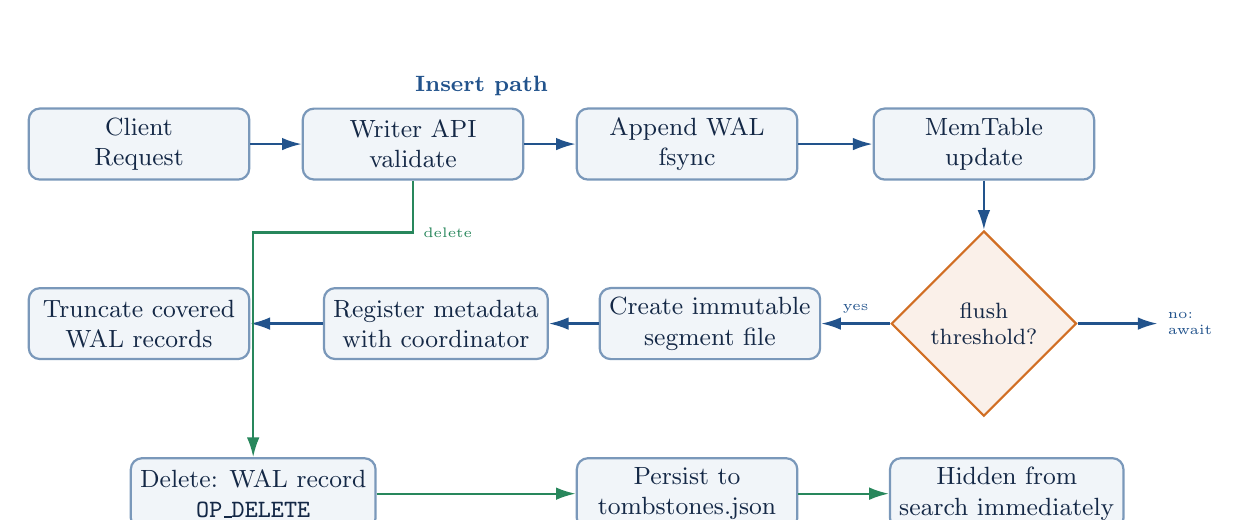
\begin{tikzpicture}[x=2.9cm, y=1.2cm,
  every node/.style={align=center}]

  %% ── Row 0: Insert path (left → right) ──────────────
  \node[flowstep] (cli)    at (0, 0) {Client\\Request};
  \node[flowstep] (wapi)   at (1.2, 0) {Writer API\\validate};
  \node[flowstep] (wal)    at (2.4, 0) {Append WAL\\fsync};
  \node[flowstep] (mem)    at (3.7, 0) {MemTable\\update};

  %% ── Row 1: Flush branch (right → left) ─────────────
  \node[decision] (thresh) at (3.7,-1.9) {flush\\threshold?};
  \node[flowstep] (seg)    at (2.5,-1.9) {Create immutable\\segment file};
  \node[flowstep] (reg)    at (1.3,-1.9) {Register metadata\\with coordinator};
  \node[flowstep] (trunc)  at (0,-1.9) {Truncate covered\\WAL records};

  %% ── Row 2: Delete branch (left → right) ────────────
  \node[flowstep] (del)    at (0.5,-3.7) {Delete: WAL record\\\texttt{OP\_DELETE}};
  \node[flowstep] (tomb)   at (2.4,-3.7) {Persist to\\tombstones.json};
  \node[flowstep] (hide)   at (3.8,-3.7) {Hidden from\\search immediately};

  %% ── Insert path arrows ──────────────────────────────
  \draw[arrow] (cli)  -- (wapi);
  \draw[arrow] (wapi) -- (wal);
  \draw[arrow] (wal)  -- (mem);
  \draw[arrow] (mem.south) -- (thresh.north);

  %% flush threshold: yes → left, no → stub right
  \draw[arrow] (thresh.west) -- node[above,font=\tiny]{yes} (seg.east);
  \draw[arrow] (seg)  -- (reg);
  \draw[arrow] (reg)  -- (trunc);
  \draw[arrow] (thresh.east) -- ++(0.35,0)
    node[right,font=\tiny,align=left]{no:\\await};

  %% ── Delete path arrows ──────────────────────────────
  %% wapi.south bends down then right to del.west
  \draw[arrowg] (wapi.south) -- ++(0,-0.55)
    node[right,font=\tiny]{delete} -| (del.north);
  \draw[arrowg] (del)  -- (tomb);
  \draw[arrowg] (tomb) -- (hide);

  %% ── Section labels ──────────────────────────────────
  \node[font=\footnotesize\bfseries,text=vsblue]  at (1.5, 0.62) {Insert path};
  % \node[font=\footnotesize\bfseries,text=vsgreen] at (2.0,-4.2) {Delete path};

\end{tikzpicture}
\caption{Write path. WAL append happens before the mutation becomes visible,
ensuring durability. Threshold-triggered flushes convert MemTable contents into
immutable FAISS-backed segments. Deletes are WAL records that are immediately
reflected in search via tombstone filtering.}
\end{figure}

\subsection{Search Flow}

\begin{figure}[H]
\centering
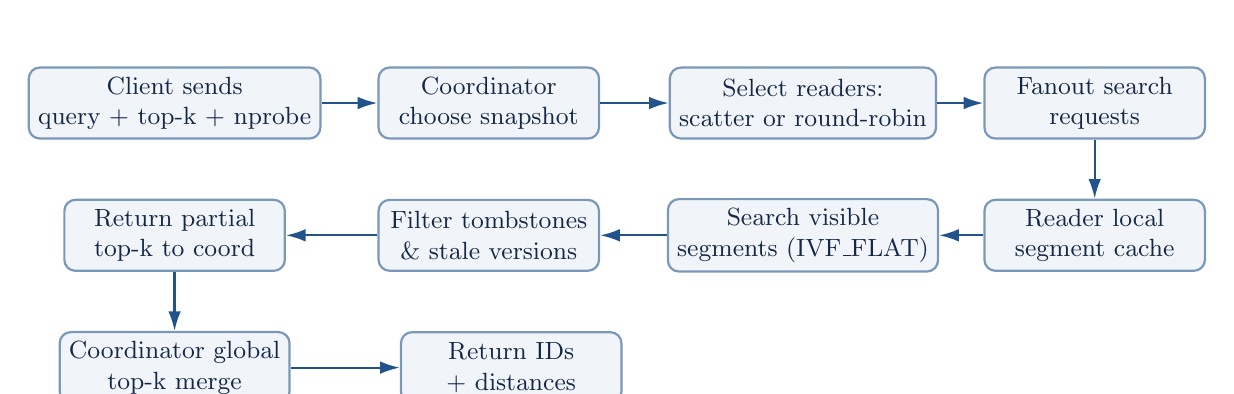
\begin{tikzpicture}[x=2.85cm, y=1.2cm,
  every node/.style={align=center}]

  %% ── Row 0: Client → Coordinator → Route → Fanout ───
  \node[flowstep] (cli)    at (0, 0) {Client sends\\query + top-k + nprobe};
  \node[flowstep] (coord)  at (1.4, 0) {Coordinator\\choose snapshot};
  \node[flowstep] (route)  at (2.8, 0) {Select readers:\\scatter or round-robin};
  \node[flowstep] (fans)   at (4.1, 0) {Fanout search\\requests};

  %% ── Row 1: Reader execution (right → left) ──────────
  \node[flowstep] (rcache) at (4.1,-1.4) {Reader local\\segment cache};
  \node[flowstep] (segs)   at (2.8,-1.4) {Search visible\\segments (IVF\_FLAT)};
  \node[flowstep] (filter) at (1.4,-1.4) {Filter tombstones\\\& stale versions};
  \node[flowstep] (part)   at (0,-1.4) {Return partial\\top-k to coord};

  %% ── Row 2: Merge and respond (left → right) ─────────
  \node[flowstep] (merge)  at (0,-2.8) {Coordinator global\\top-k merge};
  \node[flowstep] (resp)   at (1.5,-2.8) {Return IDs\\+ distances};

  %% ── Row 0 arrows ────────────────────────────────────
  \draw[arrow] (cli)   -- (coord);
  \draw[arrow] (coord) -- (route);
  \draw[arrow] (route) -- (fans);

  %% ── Down into row 1 ─────────────────────────────────
  \draw[arrow] (fans.south)   -- (rcache.north);
  \draw[arrow] (rcache.west)  -- (segs.east);
  \draw[arrow] (segs.west)    -- (filter.east);
  \draw[arrow] (filter.west)  -- (part.east);

  %% ── Down into row 2 ─────────────────────────────────
  \draw[arrow] (part.south)  -- (merge.north);
  \draw[arrow] (merge.east)  -- (resp.west);

\end{tikzpicture}
\caption{Search path. Queries execute against a consistent snapshot. Readers
search their local FAISS segment caches and return partial top-k results that
the coordinator merges into the final answer.}
\end{figure}

\subsection{WAL Recovery Flow}

\begin{figure}[H]
\centering
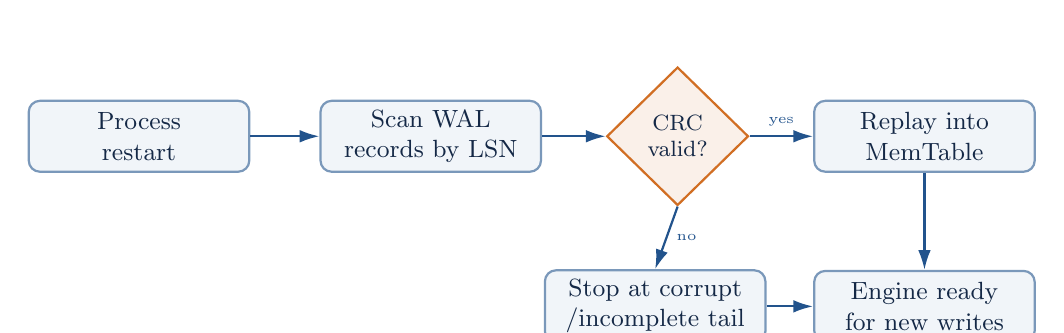
\begin{tikzpicture}[x=2.85cm, y=1.2cm,
  every node/.style={align=center}]

  %% ── Row 0: Linear happy path ────────────────────────
  \node[flowstep] (start)  at (0, 0) {Process\\restart};
  \node[flowstep] (scan)   at (1.3, 0) {Scan WAL\\records by LSN};
  \node[decision] (valid)  at (2.4, 0) {CRC\\valid?};
  \node[flowstep] (replay) at (3.5, 0) {Replay into\\MemTable};

  %% ── Row 1: Error / done path ────────────────────────
  \node[flowstep] (stop)   at (2.3,-1.8) {Stop at corrupt\\/incomplete tail};
  \node[flowstep] (ready)  at (3.5,-1.8) {Engine ready\\for new writes};

  %% ── Arrows ──────────────────────────────────────────
  \draw[arrow] (start)       -- (scan);
  \draw[arrow] (scan)        -- (valid);
  \draw[arrow] (valid.east)  -- node[above,font=\tiny]{yes} (replay.west);
  \draw[arrow] (valid.south) -- node[right,font=\tiny]{no}  (stop.north);
  \draw[arrow] (replay.south) -- (ready.north);
  \draw[arrow] (stop.east)   -- (ready.west);

\end{tikzpicture}
\caption{WAL recovery. The engine replays records newer than the latest flushed
segment. Corrupt or incomplete trailing records are ignored so partial writes do
not poison recovery.}
\end{figure}

%%%%%%%%%%%%%%%%%%%%%%%%%%%%%%%%%%%%%%%%%%%%%%%%%%%%%%%%%%%%%%%%%%%%%%%%%%%%
\section{Dataset Information}

The evaluation uses the datasets specified in the project proposal. SIFT10K is
derived from the first 10,000 SIFT1M training vectors for fast correctness and
smoke testing. SIFT1M is the primary performance benchmark. Deep1M uses
96-dimensional Deep image vectors from the public ANN-Benchmarks dataset; its
public ground truth is angular while VecScaleDB evaluates with L2.

\begin{table}[H]
\centering
\caption{Datasets used in this report.}
\renewcommand{\arraystretch}{1.2}
\begin{tabular}{lrrrrp{0.30\linewidth}}
\toprule
\textbf{Dataset} & \textbf{Train} & \textbf{Queries} & \textbf{Dim} &
\textbf{Metric} & \textbf{Purpose} \\
\midrule
SIFT10K  & 10,000    & 100   & 128 & L2 &
  Fast correctness, smoke metrics, recall sanity. \\
SIFT1M   & 1,000,000 & 1,000 & 128 & L2 &
  Primary performance and reader-scaling benchmark. \\
Deep1M   & 1,000,000 & 1,000 & 96  & L2 &
  Alternate dataset; note angular ground truth. \\
\bottomrule
\end{tabular}
\end{table}

\begin{infobox}
\textbf{Note on Deep1M recall.} The publicly available Deep1M ground truth is
computed with cosine/angular distance. Since VecScaleDB uses L2, recall
evaluation for Deep1M is skipped by default. QPS and latency measurements are
still collected.
\end{infobox}

%%%%%%%%%%%%%%%%%%%%%%%%%%%%%%%%%%%%%%%%%%%%%%%%%%%%%%%%%%%%%%%%%%%%%%%%%%%%
\section{Benchmark Methodology}

\subsection{Measured Quantities}

Each benchmark run collects:
\begin{itemize}[noitemsep,topsep=4pt]
  \item load time and vectors inserted per second,
  \item total completed search queries, error count, and QPS,
  \item p50, p95, and p99 search latency (ms),
  \item recall@10 where compatible ground truth exists,
  \item QPS-vs-reader-count for 1–5 readers (scaling evaluation).
\end{itemize}

\subsection{Key Commands}

\begin{lstlisting}[language=bash, caption={Run full automated test suite.}]
venv/bin/python -m pytest tests -q
# Expected: 71 passed, 2 warnings
\end{lstlisting}

\begin{lstlisting}[language=bash, caption={Run proposal feature suite only.}]
venv/bin/python -m pytest tests/feature -q
# Expected: 17 passed, 2 warnings
\end{lstlisting}

\begin{lstlisting}[language=bash, caption={Load SIFT1M into a live distributed cluster.}]
docker compose down && docker compose up -d --build

python -m vecscaledb.bench.load_dataset \
  --dataset data/sift1m/sift1m.hdf5 \
  --writer-url http://127.0.0.1:8100 \
  --batch-size 10000
\end{lstlisting}

\begin{lstlisting}[language=bash, caption={Run QPS benchmark (60 s, 32 concurrent workers).}]
python -m vecscaledb.bench.benchmark_qps \
  --dataset data/sift1m/sift1m.hdf5 \
  --coordinator-url http://127.0.0.1:8000 \
  --query-limit 1000 --top-k 10 --nprobe 32 \
  --concurrency 32 --duration 60
\end{lstlisting}

\begin{lstlisting}[language=bash, caption={Reader scaling sweep (1–5 readers, auto-scale).}]
python -m vecscaledb.bench.scaling_eval \
  --dataset data/sift1m/sift1m.hdf5 \
  --coordinator-url http://127.0.0.1:8000 \
  --reader-counts 1 2 3 4 5 \
  --duration 60 --concurrency 32 \
  --output scaling_results.json --auto-scale
\end{lstlisting}

\begin{lstlisting}[language=bash, caption={Generate all benchmark metrics and compile report.}]
bash report/run_all_dataset_metrics.sh
bash report/run_sift1m_scaling.sh
\end{lstlisting}

%%%%%%%%%%%%%%%%%%%%%%%%%%%%%%%%%%%%%%%%%%%%%%%%%%%%%%%%%%%%%%%%%%%%%%%%%%%%
\section{Benchmark Results}

\subsection{Load Throughput}

\begin{table}[H]
\centering
\caption{Dataset loading results.}
\renewcommand{\arraystretch}{1.2}
\begin{tabular}{lrrrr}
\toprule
\textbf{Dataset} & \textbf{Inserted} & \textbf{Load time (s)} &
\textbf{Vectors/s} & \textbf{Segments} \\
\midrule
SIFT10K & 10,000    & 1.07   & 9{,}330.91 & 1  \\
SIFT1M  & 1,000,000 & 103.06 & 9{,}703.23 & 20 \\
Deep1M  & 1,000,000 & 129.65 & 7{,}712.84 & 20 \\
\bottomrule
\end{tabular}
\end{table}

\begin{figure}[H]
\centering
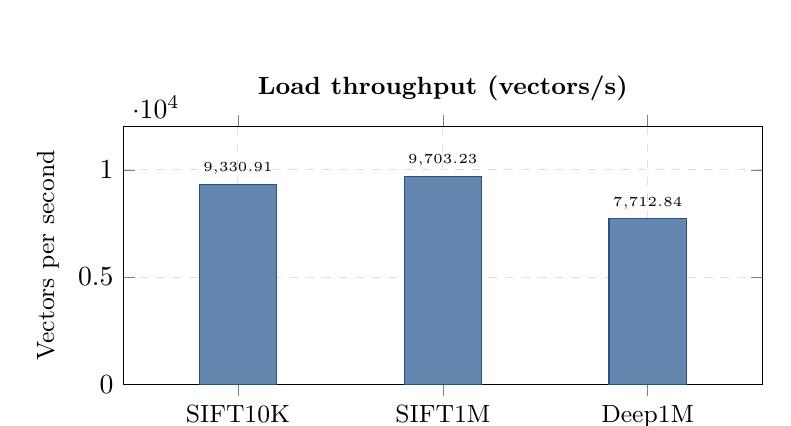
\begin{tikzpicture}
\begin{axis}[
  ybar, width=0.80\textwidth, height=0.40\textwidth,
  ylabel={Vectors per second}, ylabel style={font=\small},
  symbolic x coords={SIFT10K,SIFT1M,Deep1M},
  xtick=data, xticklabel style={font=\small},
  nodes near coords, nodes near coords align={vertical},
  nodes near coords style={font=\tiny},
  ymin=0, ymax=12000,
  bar width=28pt,
  enlarge x limits=0.28,
  grid=major, grid style={dashed,gray!25},
  title={Load throughput (vectors/s)}, title style={font=\small\bfseries}
]
\addplot[fill=vsblue!70, draw=vsblue] coordinates {
  (SIFT10K,9330.91) (SIFT1M,9703.23) (Deep1M,7712.84)
};
\end{axis}
\end{tikzpicture}
\caption{Load throughput. SIFT10K and SIFT1M use 128-dimensional float32
vectors; Deep1M uses 96-dimensional vectors and a different HDF5 layout,
resulting in lower throughput in this environment.}
\end{figure}

\subsection{Search Throughput and Latency}

\begin{table}[H]
\centering
\caption{Search metrics from a single benchmark run.}
\renewcommand{\arraystretch}{1.2}
\begin{tabular}{lrrrrrr}
\toprule
\textbf{Dataset} & \textbf{Queries} & \textbf{Errors} & \textbf{QPS} &
\textbf{p50 (ms)} & \textbf{p95 (ms)} & \textbf{p99 (ms)} \\
\midrule
SIFT10K & 6{,}607 & 0 & 109.77 & 294.89 & 357.88 & 387.10 \\
SIFT1M  & 5{,}250 & 0 & 87.29  & 363.78 & 433.02 & 487.44 \\
Deep1M  & 5{,}334 & 0 & 88.67  & 358.52 & 432.01 & 501.62 \\
\bottomrule
\end{tabular}
\end{table}

\begin{figure}[H]
\centering
\begin{subfigure}{0.47\textwidth}
\centering
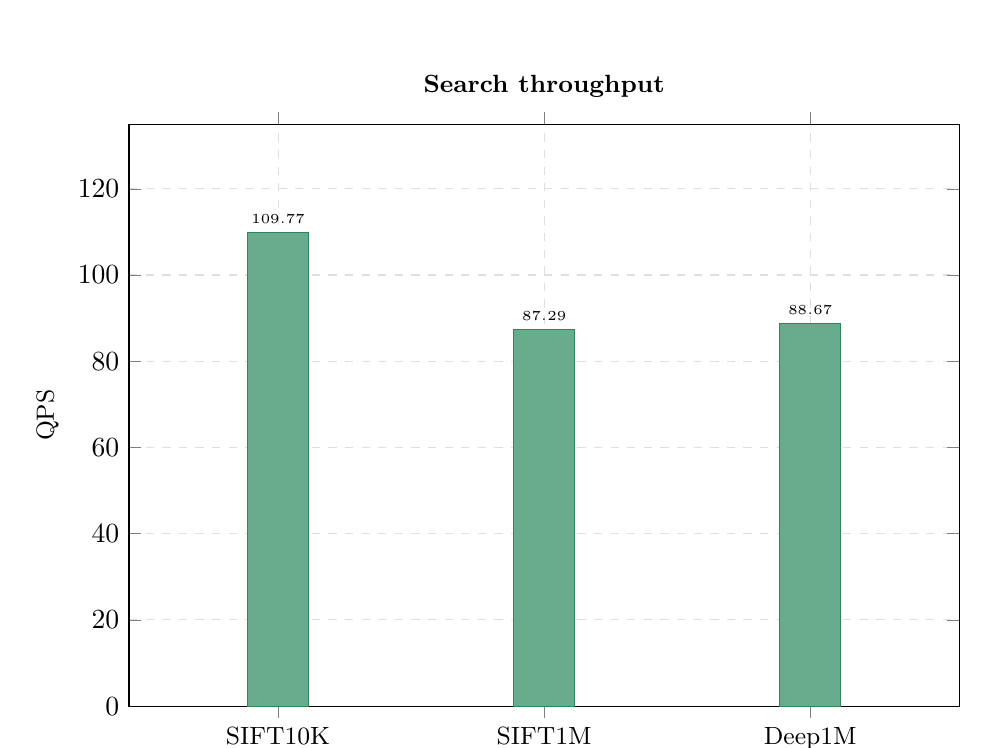
\begin{tikzpicture}
\begin{axis}[
  ybar, width=\textwidth, height=0.74\textwidth,
  ylabel={QPS}, ylabel style={font=\small},
  symbolic x coords={SIFT10K,SIFT1M,Deep1M},
  xtick=data, xticklabel style={font=\small},
  nodes near coords, nodes near coords style={font=\tiny},
  ymin=0, ymax=135,
  bar width=22pt,
  enlarge x limits=0.28,
  grid=major, grid style={dashed,gray!25},
  title={Search throughput}, title style={font=\small\bfseries}
]
\addplot[fill=vsgreen!70, draw=vsgreen] coordinates {
  (SIFT10K,109.77) (SIFT1M,87.29) (Deep1M,88.67)
};
\end{axis}
\end{tikzpicture}
\caption{QPS by dataset.}
\end{subfigure}
\hfill
\begin{subfigure}{0.47\textwidth}
\centering
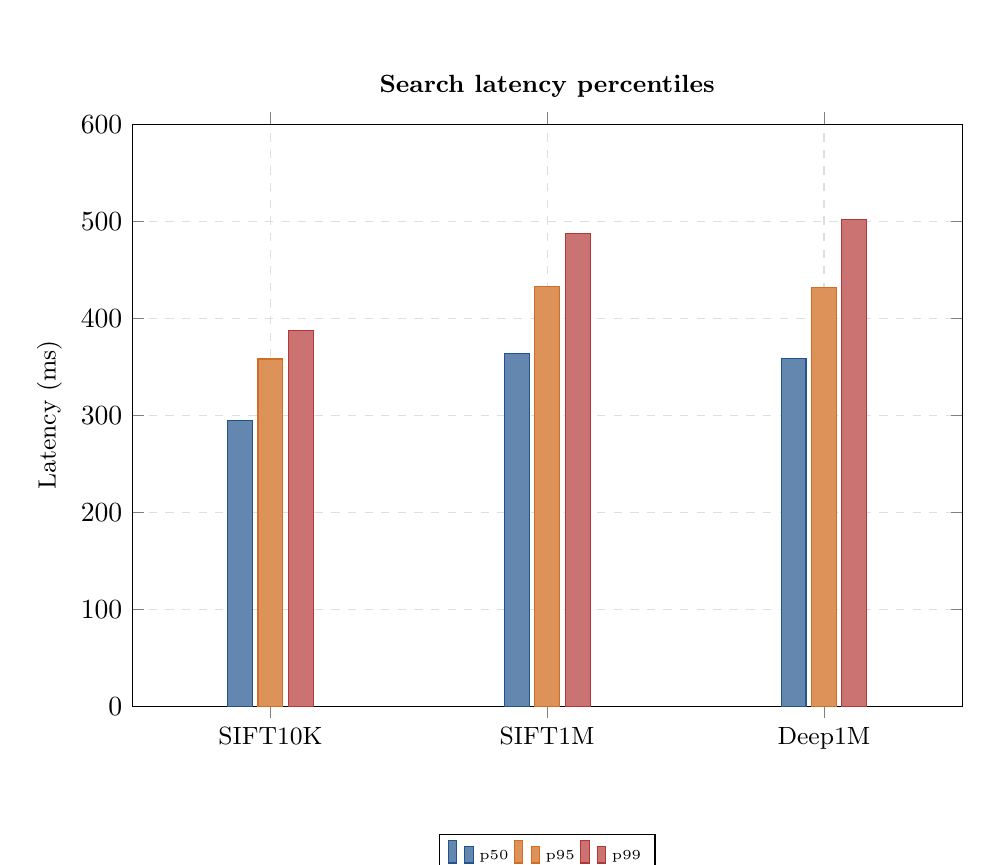
\begin{tikzpicture}
\begin{axis}[
  ybar, width=\textwidth, height=0.74\textwidth,
  ylabel={Latency (ms)}, ylabel style={font=\small},
  symbolic x coords={SIFT10K,SIFT1M,Deep1M},
  xtick=data, xticklabel style={font=\small},
  ymin=0, ymax=600,
  bar width=9pt,
  enlarge x limits=0.25,
  legend style={at={(0.5,-0.22)}, anchor=north, legend columns=3,
                font=\tiny},
  grid=major, grid style={dashed,gray!25},
  title={Search latency percentiles}, title style={font=\small\bfseries}
]
\addplot[fill=vsblue!70,  draw=vsblue]   coordinates {(SIFT10K,294.89) (SIFT1M,363.78) (Deep1M,358.52)};
\addplot[fill=vsorange!75,draw=vsorange] coordinates {(SIFT10K,357.88) (SIFT1M,433.02) (Deep1M,432.01)};
\addplot[fill=vsred!70,   draw=vsred]    coordinates {(SIFT10K,387.10) (SIFT1M,487.44) (Deep1M,501.62)};
\legend{p50, p95, p99}
\end{axis}
\end{tikzpicture}
\caption{Latency percentiles.}
\end{subfigure}
\caption{Search performance across datasets. SIFT10K achieves higher QPS due to
the smaller indexed corpus. SIFT1M and Deep1M are comparable.}
\end{figure}

\subsection{Recall}

\begin{table}[H]
\centering
\caption{Recall evaluation results (nprobe=32, top-k=10).}
\renewcommand{\arraystretch}{1.2}
\begin{tabular}{lrrrr p{0.32\linewidth}}
\toprule
\textbf{Dataset} & \textbf{Queries} & \textbf{nprobe} &
\textbf{Lat (ms)} & \textbf{R@10} & \textbf{Notes} \\
\midrule
SIFT10K & 100   & 32 & 15.88 & 0.104  & R@100 = 0.0248; small 10K IVF index. \\
SIFT1M  & 1,000 & 32 & 28.04 & 0.9977 & R@100 = 0.9960; excellent recall at nprobe=32. \\
Deep1M  & ---   & --- & ---   & ---    & Angular ground truth; L2 recall skipped. \\
\bottomrule
\end{tabular}
\end{table}

\begin{infobox}
\textbf{Note on SIFT10K recall.} The recall figure of 0.104 at nprobe=32
reflects a small trained IVF index over only 10\,K vectors with a relatively
large number of IVF cells. Recall improves with larger corpora.

\textbf{SIFT1M recall.} With \texttt{nprobe=32} over the full 1\,M-vector
corpus, VecScaleDB achieves \textbf{R@10 = 0.9977} and R@100 = 0.9960 on
1,000 queries, measured against the L2 ground truth. This demonstrates
high-fidelity approximate nearest-neighbour retrieval at scale.

\textbf{Deep1M recall} is skipped because the public ANN-Benchmarks ground
truth for Deep is angular while VecScaleDB evaluates with L2.
\end{infobox}

\subsection{Reader Scaling}

\begin{table}[H]
\centering
\caption{QPS scaling with 1–5 readers.}
\renewcommand{\arraystretch}{1.2}
\setlength{\tabcolsep}{6pt}
\begin{tabular}{rrrrrr}
\toprule
\textbf{Readers} & \textbf{S1M QPS} & \textbf{S1M p99} &
\textbf{D1M QPS} & \textbf{D1M p99} & \textbf{D1M err} \\
\midrule
1 & 100.50 & 513.91 & 104.18 & 459.69 & 0 \\
2 & 98.03  & 473.58 & 97.75  & 447.68 & 0 \\
3 & 93.86  & 491.42 & 94.39  & 453.80 & 0 \\
4 & 89.87  & 489.28 & 84.63  & 569.49 & 0 \\
5 & 86.20  & 486.23 & 83.12  & 522.39 & 0 \\
\bottomrule
\end{tabular}
\end{table}

\begin{figure}[H]
\centering
\begin{subfigure}{0.47\textwidth}
\centering
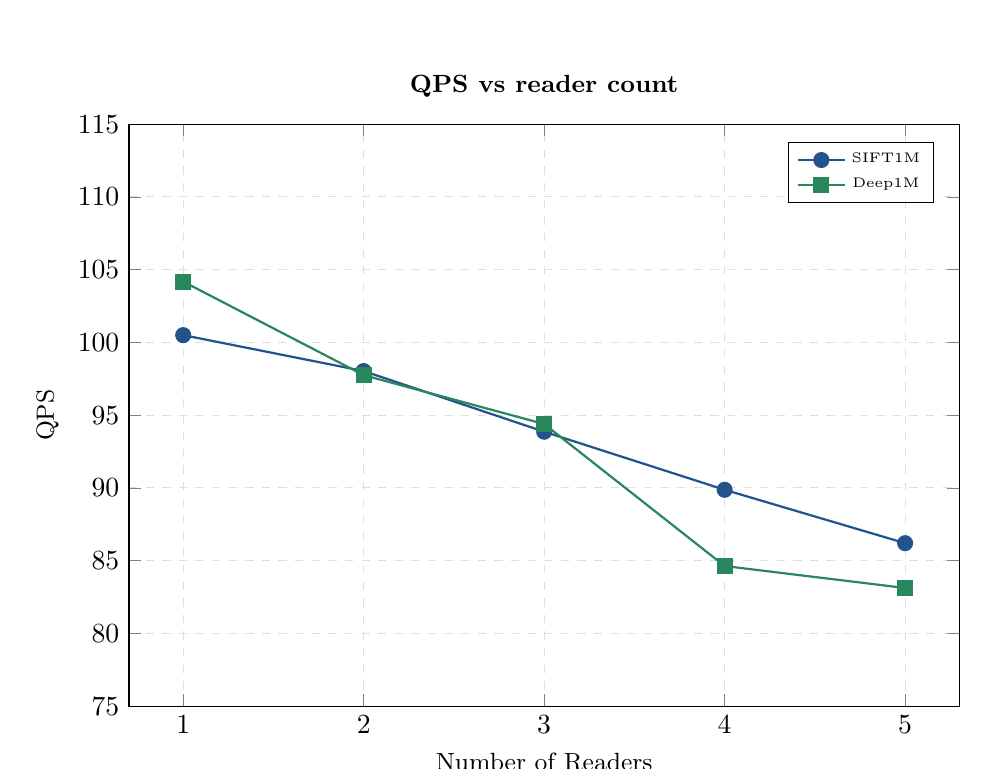
\begin{tikzpicture}
\begin{axis}[
  width=\textwidth, height=0.74\textwidth,
  xlabel={Number of Readers}, xlabel style={font=\small},
  ylabel={QPS}, ylabel style={font=\small},
  xmin=0.7, xmax=5.3,
  xtick={1,2,3,4,5},
  ymin=75, ymax=115,
  legend pos=north east, legend style={font=\tiny},
  grid=major, grid style={dashed,gray!25},
  title={QPS vs reader count}, title style={font=\small\bfseries}
]
\addplot[color=vsblue, mark=*, thick, mark size=2.5pt]
  coordinates {(1,100.50)(2,98.03)(3,93.86)(4,89.87)(5,86.20)};
\addplot[color=vsgreen, mark=square*, thick, mark size=2.5pt]
  coordinates {(1,104.18)(2,97.75)(3,94.39)(4,84.63)(5,83.12)};
\legend{SIFT1M, Deep1M}
\end{axis}
\end{tikzpicture}
\caption{QPS vs reader count.}
\end{subfigure}
\hfill
\begin{subfigure}{0.47\textwidth}
\centering
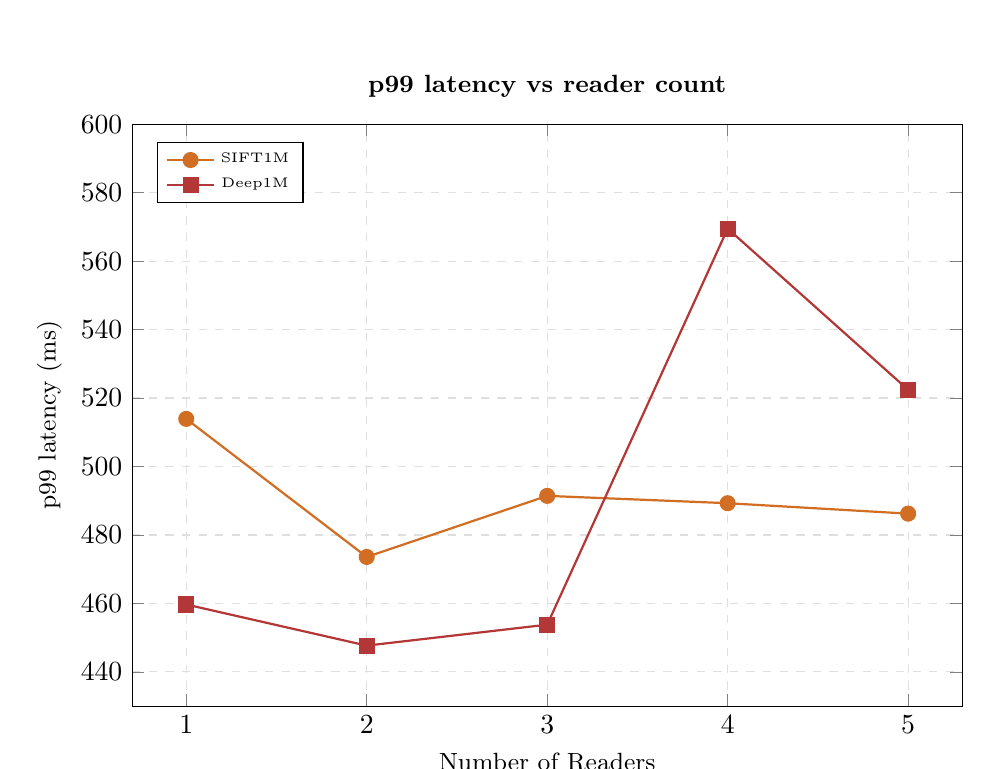
\begin{tikzpicture}
\begin{axis}[
  width=\textwidth, height=0.74\textwidth,
  xlabel={Number of Readers}, xlabel style={font=\small},
  ylabel={p99 latency (ms)}, ylabel style={font=\small},
  xmin=0.7, xmax=5.3,
  xtick={1,2,3,4,5},
  ymin=430, ymax=600,
  legend pos=north west, legend style={font=\tiny},
  grid=major, grid style={dashed,gray!25},
  title={p99 latency vs reader count}, title style={font=\small\bfseries}
]
\addplot[color=vsorange, mark=*, thick, mark size=2.5pt]
  coordinates {(1,513.91)(2,473.58)(3,491.42)(4,489.28)(5,486.23)};
\addplot[color=vsred, mark=square*, thick, mark size=2.5pt]
  coordinates {(1,459.69)(2,447.68)(3,453.80)(4,569.49)(5,522.39)};
\legend{SIFT1M, Deep1M}
\end{axis}
\end{tikzpicture}
\caption{p99 latency vs reader count.}
\end{subfigure}
\caption{Reader scaling behaviour. QPS decreases with reader count in this
single-machine environment due to CPU contention, replicated search overhead,
and shared-storage access pressure. SIFT1M declines from 100.50 QPS at one
reader to 86.20 at five. Deep1M follows a similar trend. The architecture is
correct; scaling limits are environmental.}
\end{figure}

%%%%%%%%%%%%%%%%%%%%%%%%%%%%%%%%%%%%%%%%%%%%%%%%%%%%%%%%%%%%%%%%%%%%%%%%%%%%
\section{Correctness and Feature Tests}

\subsection{Test Suite Overview}

\begin{lstlisting}[language=bash, caption={Full and feature-only test suites.}]
# Full suite
venv/bin/python -m pytest tests -q
# 71 passed, 2 warnings

# Proposal feature suite
venv/bin/python -m pytest tests/feature -q
# 17 passed, 2 warnings
\end{lstlisting}

\begin{longtable}{p{0.25\linewidth} p{0.65\linewidth}}
\caption{Feature tests and what they prove.}\\
\toprule
\textbf{Test area} & \textbf{Validation} \\
\midrule
\endfirsthead
\toprule
\textbf{Test area} & \textbf{Validation} \\
\midrule
\endhead
IVF\_FLAT and segments &
  External IDs, nprobe search, exact self-match (distance = 0), save/load
  persistence, segment metadata arrays, and segment searchability after
  reload. \\
\midrule
WAL and recovery &
  Valid records replay after restart; corrupt trailing checksum is
  silently ignored; acknowledged unflushed writes survive a simulated
  process crash. \\
\midrule
Deletes and updates &
  Tombstones survive flush and engine restart; reader caches hide deleted
  IDs; reinserting the same ID hides stale segment versions. \\
\midrule
Snapshot isolation &
  Old snapshots do not observe newer MemTable writes; current snapshot
  does. Both segment visibility and MemTable visibility are filtered by
  the same snapshot ID. \\
\midrule
Reader recovery &
  A restarted reader starts with an empty cache, fetches segment metadata
  from the coordinator, reloads files from shared storage, and returns
  the same search results as before the restart. \\
\midrule
Distribution &
  Writer sharding (\texttt{id \% num\_shards}), scatter-gather merge,
  all-shard replicated loading, consistent hash ring routing and
  rebalancing, and coordinator-client round-robin failover. \\
\midrule
Observability &
  Metrics registry records request totals, search latency histograms,
  and runtime gauges for MemTable size, segment count, and WAL LSN. \\
\bottomrule
\end{longtable}

\subsection{Key Feature Explanations}

\subsubsection{IVF\_FLAT Vector Search}

\texttt{IVFFlatIndex.train()} trains a FAISS IVF\_FLAT index. Add operations
store vectors using external integer IDs. Search accepts \texttt{top\_k} and
\texttt{nprobe}; \texttt{nprobe} controls how many Voronoi cells are probed.
Tiny segments (fewer vectors than cells) automatically fall back to exact
\texttt{IndexFlatL2} to avoid unreliable FAISS training.

\subsubsection{WAL Durability}

\texttt{WAL.append()} writes insert/delete records with LSN, operation type,
IDs, vectors, and CRC32 checksum before the MemTable is mutated.
\texttt{WAL.recover()} replays records whose LSN is newer than the latest
flushed segment's snapshot ID, stopping at the first corrupt or incomplete
trailing record.

\subsubsection{Snapshot Isolation}

\texttt{Snap\-shot\-Ma\-na\-ger.cre\-ate\_snap\-shot(current\_lsn)} creates a read
timestamp. \texttt{vis\-i\-ble\_seg\-ments()} allows only segments whose
\texttt{snap\-shot\_id $\leq$ read\_snap\-shot}.
\texttt{Mem\-Ta\-ble.to\_ar\-rays(snap\-shot\_id)} hides entries newer than the
snapshot. Together, a query cannot observe half of an in-progress write.

\subsubsection{Scatter-Gather vs. Replicated Modes}

In \emph{scatter-gather} mode each reader owns one shard (\texttt{id \%
num\_shards}) and the coordinator fans the query to all readers, then merges
partial top-k results. In \emph{replicated} mode every reader loads all shards
and the coordinator round-robins requests for QPS scaling.

%%%%%%%%%%%%%%%%%%%%%%%%%%%%%%%%%%%%%%%%%%%%%%%%%%%%%%%%%%%%%%%%%%%%%%%%%%%%
\section{Fault Tolerance}

\subsection{Fault-Tolerance Matrix}

\begin{table}[H]
\centering
\caption{Failure scenarios and recovery mechanisms.}
\renewcommand{\arraystretch}{1.3}
\begin{tabular}{p{0.20\linewidth} p{0.42\linewidth} p{0.28\linewidth}}
\toprule
\textbf{Failure} & \textbf{Recovery mechanism} & \textbf{Covering test} \\
\midrule
Writer crash &
  WAL replay; MemTable rebuilt from records newer than last segment. &
  \small\texttt{test\_lsm\_\ldots{} crash\_recovery} \\
Reader crash &
  New process fetches segment list from coordinator; reloads files from shared storage. &
  \small\texttt{test\_reader\_api \ldots{} restart} \\
Coordinator leader crash &
  etcd TTL expires; another coordinator campaigns. &
  \small\texttt{test\_etcd \ldots{} ttl\_failover} \\
Coordinator unreachable &
  Client retries across replica URLs. &
  \small\texttt{test\_coordinator \ldots{} failover} \\
Corrupt WAL tail &
  Recovery stops at first bad CRC; only committed records are visible. &
  \small\texttt{test\_wal\_recovers \ldots{} tail} \\
\bottomrule
\end{tabular}
\end{table}

\subsection{Manual Fault-Tolerance Commands}

\begin{lstlisting}[language=bash, caption={Reader restart check.}]
docker compose stop reader-3
docker compose start reader-3
sleep 15
curl http://127.0.0.1:8203/ready
\end{lstlisting}

\begin{lstlisting}[language=bash, caption={Coordinator failover check.}]
docker compose stop coordinator-0
sleep 15
curl http://127.0.0.1:8001/health          # coordinator-1 still serves
python - <<'PY'
import httpx
query = [1.0] + [0.0]*127
print(httpx.post("http://127.0.0.1:8001/search",
      json={"query": query, "top_k": 5, "nprobe": 32}).json())
PY
docker compose start coordinator-0
\end{lstlisting}

\begin{lstlisting}[language=bash, caption={Writer restart check.}]
docker compose stop writer-0
docker compose start writer-0
sleep 10
curl http://127.0.0.1:8100/health
\end{lstlisting}

%%%%%%%%%%%%%%%%%%%%%%%%%%%%%%%%%%%%%%%%%%%%%%%%%%%%%%%%%%%%%%%%%%%%%%%%%%%%
\section{Discussion}

\subsection{What Works}

\begin{itemize}[noitemsep,topsep=4pt]
  \item The durability path is complete: WAL append $\to$ MemTable update
    $\to$ flush $\to$ segment persistence $\to$ WAL truncation.
  \item The read path is snapshot-aware and filters deletes and stale
    duplicate versions without waiting for compaction.
  \item Reader processes recover from shared storage without owning data
    permanently, making reader crash recovery lightweight.
  \item The coordinator supports both scatter-gather and replicated reader
    modes, covering both the correctness and the throughput use cases.
  \item The Docker topology (3 coordinators, 1 writer, 5 readers, etcd)
    matches the promised distributed cluster shape.
  \item A consistent hash ring manages reader node membership and can absorb
    add/remove events while maintaining routing correctness.
\end{itemize}

\subsection{Observed Benchmark Behaviour}

The measured scaling curve does not show near-linear speedup. SIFT1M QPS
decreases from 100.50 at one reader to 86.20 at five readers. Deep1M declines
from 104.18 at one reader to 83.12 at five. This is attributable to:

\begin{itemize}[noitemsep,topsep=4pt]
  \item \textbf{CPU contention:} all services run on the same host.
  \item \textbf{Replicated search overhead:} in replicated mode every reader
    loads and searches all segments; fanout cost grows with reader count.
  \item \textbf{Shared-storage pressure:} multiple readers compete for the
    same volume I/O on startup and cache refresh.
  \item \textbf{Network/container overhead:} localhost TCP between
    coordinator and readers adds latency at high concurrency.
\end{itemize}

The architecture correctness is not affected by these environmental limits.

\subsection{Known Caveats}

\begin{itemize}[noitemsep,topsep=4pt]
  \item There is no separate \texttt{/update} endpoint. Updates are
    implemented as reinsertion of the same external ID; search suppresses
    older segment versions.
  \item Tiny or undertrained segments use exact \texttt{IndexFlatL2} search
    instead of IVF training to avoid FAISS training failures when the
    vector count is below the cluster count.
  \item Deep1M recall is skipped by default because the public ground truth
    is angular while the engine evaluates L2.
  \item Unit and integration tests do not start Docker. Full cluster
    behaviour must be demonstrated separately during evaluation.
\end{itemize}

%%%%%%%%%%%%%%%%%%%%%%%%%%%%%%%%%%%%%%%%%%%%%%%%%%%%%%%%%%%%%%%%%%%%%%%%%%%%
\section{Conclusion}

VecScaleDB implements all core proposal features: distributed architecture,
FAISS-backed vector similarity search, dynamic data management (insert, delete,
update-via-reinsert), snapshot isolation, fault tolerance, and a five-reader
Docker evaluation setup. The 71-test suite validates each distributed mechanism
in isolation, while the 17-test feature suite maps directly to proposal claims.

The most important evaluation result is that correctness is fully established.
The observed QPS scaling curve is flat-to-declining in the local single-machine
benchmark environment, which is expected and explained by CPU contention and
replicated reader overhead rather than an architectural defect.

%%%%%%%%%%%%%%%%%%%%%%%%%%%%%%%%%%%%%%%%%%%%%%%%%%%%%%%%%%%%%%%%%%%%%%%%%%%%
\appendix
\section{Runtime Setup Reference}

\begin{lstlisting}[language=bash, caption={First-time setup.}]
python3 -m venv venv
source venv/bin/activate
python -m pip install --upgrade pip
python -m pip install -r requirements.txt
python -m pip install -e .
\end{lstlisting}

\begin{lstlisting}[language=bash, caption={Single-node mode (insert + search on port 8000).}]
python -m vecscaledb.node
curl http://127.0.0.1:8000/health
# API docs: http://127.0.0.1:8000/docs
\end{lstlisting}

\begin{lstlisting}[language=bash, caption={Start full distributed cluster.}]
docker compose down
unset VECSCALE_SEGMENT_FLUSH_THRESHOLD
docker compose up -d --build
docker compose ps
\end{lstlisting}

\begin{lstlisting}[language=bash, caption={Quick distributed demo (flush every 2 vectors).}]
VECSCALE_SEGMENT_FLUSH_THRESHOLD=2 docker compose up -d --build
# Insert two 128-d vectors into writer, then search via coordinator.
\end{lstlisting}

\begin{lstlisting}[language=bash, caption={Scatter-gather shard mode.}]
docker compose -f docker-compose.yml -f docker-compose.scatter.yml up -d --build
\end{lstlisting}

\section{Key Source Paths}

\begin{lstlisting}
vecscaledb/coordinator/app.py    coordinator REST API and fanout
vecscaledb/coordinator/ring.py   consistent hash ring
vecscaledb/writer/pipeline.py    LSM pipeline and shard assignment
vecscaledb/writer/app.py         writer REST API
vecscaledb/reader/search.py      reader segment cache and search
vecscaledb/storage/lsm.py        LSM engine (insert/delete/flush)
vecscaledb/storage/wal.py        WAL append and recovery
vecscaledb/storage/snapshot.py   snapshot manager
vecscaledb/index/ivf_flat.py     FAISS IVF_FLAT wrapper
vecscaledb/index/segment.py      immutable segment create/load
tests/feature/                   proposal-level feature tests
report/results/                  benchmark JSON outputs
\end{lstlisting}

\section{Health Check Commands}

\begin{lstlisting}[language=bash, caption={Health and readiness checks for all services.}]
curl http://127.0.0.1:8000/health   # coordinator-0
curl http://127.0.0.1:8001/health   # coordinator-1
curl http://127.0.0.1:8002/health   # coordinator-2
curl http://127.0.0.1:8100/health   # writer-0
curl http://127.0.0.1:8200/ready    # reader-0
curl http://127.0.0.1:8201/ready    # reader-1
curl http://127.0.0.1:8202/ready    # reader-2
curl http://127.0.0.1:8203/ready    # reader-3
curl http://127.0.0.1:8204/ready    # reader-4
# Metrics
curl http://127.0.0.1:8000/metrics
curl http://127.0.0.1:8100/metrics
\end{lstlisting}

\end{document}
